\chapter{Confronto tra Client e Server}\label{cap:scalprocont}
\section{Scalabilit\`a}\label{sez:scalabilita}
La Scalabilit\`a, ossia la capacit\`a dell'applicazione di resistere all'aumentare del numero di utenti concorrenti che ne usufruiscono, dipende fortemente dal modello scelto, come anche dalla tipologia di applicazione sviluppata.
Quindi scegliere il modello pi\`u adatto non \`e banale e non ne esiste uno standard sempre corretto.

Il problemi introdotti dalla scalabilit\`a comunque sono fondamentalmente diversi tra Blazor Server, e tutti gli altri modelli.
Questo principalmente per 3 motivi:
\begin{enumerate}
	\item Blazor Server delega completamente al server che ospita l'applicazione il carico computazionale necessario per gestire ogni singolo evento della UI di ogni sessione per ogni utente connesso, compreso il salvataggio in memoria RAM dello stato di ciascuna UI durante l'utilizzo dell'applicazione, visto che ad ogni browser coinvolto, dopo l'inizializzazione, arrivano solamente le minime differenze necessarie per effettuare il render della UI rispetto al frame precedente, ogni volta che deve cambiare qualcosa.
	Ci\`o implica che la potenza del server debba tener conto di eventuali picchi di utenze, e debba avere a disposizione sufficiente RAM per poter mantenere in memoria lo stato dell'applicazione di ciascun utente concorrente connesso.
	
	\item Il secondo \`e che Blazor Server, necessita di almeno una connessione costante ed affidabile con ogni sessione di ogni utente collegato.
	
	\item Il terzo \`e che questo modello sfrutta SignalR, che per funzionare al meglio utilizza il protocollo di trasporto WebSocket, quindi la macchina server sul quale viene ospitata l'applicazione Blazor \`e consigliato che lo supporti, pur non essendo necessario.
\end{enumerate}

Gli altri modelli invece sfruttano l'hardware di ogni client connesso, come solitamente avviene per le SPA odierne.
Sono quindi in linea con il comportamento degli altri framework basati su Javascript come Angular o React, in particolare Blazor WebAssembly. 
Di seguito verranno quindi confrontati pro e contro dell'utilizzo del modello Blazor Server e del modello Blazor WebAssembly, partendo dai punti evidenziati nella figura \ref{fig:blazorModelsProCons}.
\begin{figure}[H]
	\centerline{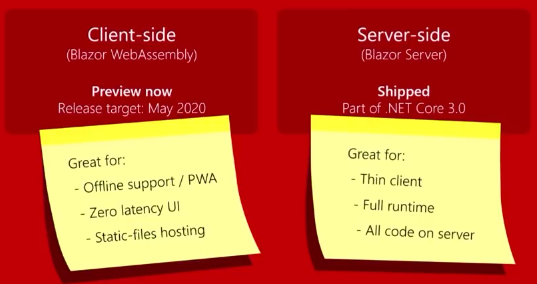
\includegraphics[scale=0.8]{figure/ClientServerProCons.png}}
	\caption{Confronto Modelli Client-Server}
	\label{fig:blazorModelsProCons}
\end{figure}

\section{Blazor Server}\label{sez:scalabilitaBServer}
\subsection{Pro}\label{sez:proBServer}
Blazor Server vanta, come primo punto a favore, il fatto di essere stato creato per essere una soluzione completa, ma che pu\`o essere utilizzata in modo complementare in applicazioni gi\`a esistenti che ad esempio si basano su Razor.
Si pu\`o quindi andare ad ampliare queste applicazioni senza doverle riscrivere da zero.
In questo modo si possono continuare a sfruttare le pagine completamente renderizzate lato server dove necessario, ma si possono anche gestire le interazioni del client con la UI potendo referenziare codice C\# senza doverlo riscrivere in Javascript o anche solo passare tramite JS, in parti dell'applicazione dove si ritiene sia pi\`u adatto farlo.

Un altro grande pro di questo modello \`e il fatto di poter delegare al server la responsabilit\`a di dover sopportare un peso maggiore, al crescere dell'applicazione, mentre il client non deve scaricare pi\`u dati.
Infatti i file scaricati lato client sono solo quelli necessari all'inizializzazione della UI e allo stabilimento di una connessione con il server, che quindi al crescere del peso dell'applicazione, non invia dati in pi\`u ai client, ma continua solamente a inviare le differenze della UI rispetto allo stato precedente.
Questo secondo vantaggio, rende il modello ideale per i casi in cui si deve creare un'applicazione per nella quale i client che la utilizzeranno potrebbero avere a disposizione computer o cellulari a basso costo.

Il terzo punto a favore, molto utile durante lo sviluppo di applicazioni \`e che il codice dinamico relativo alla logica dell'applicazione sviluppata, comprese eventuali logiche di business, non escono mai dal server, in quanto tutto viene eseguito lato server dopo la connessione iniziale.

Il quarto punto a favore, \`e che se si vuole sviluppare un'applicazione Blazor da utilizzare in produzione, fino a maggio 2020 questo modello \`e l'unico ad essere ufficialmente supportato e che si pu\`o quindi cominciare gi\`a ad utilizzare.

Un quinto punto a favore, \`e che essendo questo modello pronto per produzione, si trovano gi\`a oggi diverse guide online di utenti che hanno provato ad utilizzarlo e che si sono scontrati con i principali problemi esistenti, e in caso di problemi si pu\`o eseguire il debug del codice scritto utilizzando Visual Studio 2019 o Visual Studio Code o ricevere supporto ufficiale da Microsoft nel caso si trovi un problema negli strumenti che si hanno a disposizione.

Infine il fatto che l'applicazione esegua sul server, implica che si possa utilizzare l'intero runtime di .NET Core, che implementa completamente il .NET Standard 2.0.
\subsection{Contro}\label{sez:controBServer}
Il principale punto a sfavore di Blazor Server \`e la gi\`a citata RAM consumata da ogni UI per ogni sessione di ogni utente che utilizza l'applicazione.
Un benchmark eseguito da Microsoft a tal proposito, ha mostrato come il principale collo di bottiglia di un'applicazione Blazor sia proprio la RAM.
Microsoft ha dichiarato che hanno stimato vengano occupati in media 250 KB in RAM per ogni nuova connessione di un utente ad un'applicazione base di tipo "hello world" e consigliano di dedicare almeno 273 KB per utente se non si ha chiaro da dove partire.Durante il test di carico svolto da Microsoft \`e stata utilizzata una sola macchina virtuale Azure di fascia medio-bassa(Standard D1V2)come server per ospitare l'applicazione Blazor, avendo quindi a disposizione 3.5 GB di RAM e le caratteristiche visibili in figura \ref{fig:vmStandardD1V2}.

\begin{figure}[H]
	\centerline{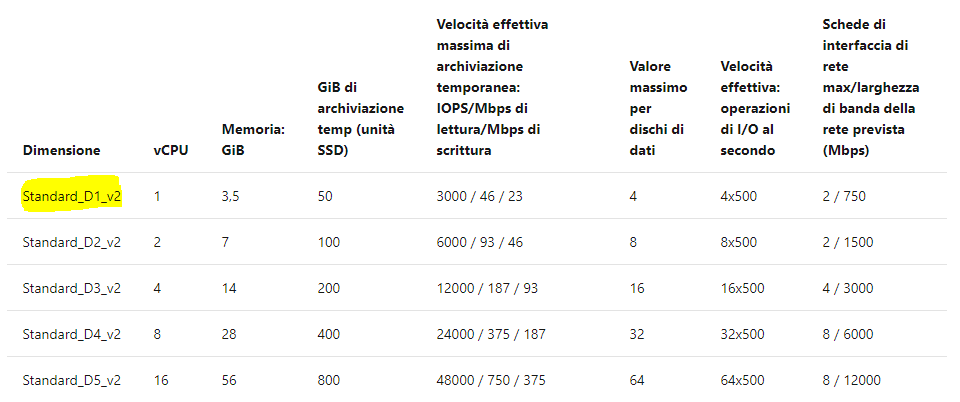
\includegraphics[scale=0.5]{figure/Standard_D1_V2.PNG}}
	\caption{Parametri VM utilizzata per il test di carico}
	\label{fig:vmStandardD1V2}
\end{figure}

Con questi parametri, l'applicazione \`e stata in grado di gestire 5000 utenti concorrenti senza perdita significativa di performance \cite{blazorModelsScenarios} \cite{bServerConcurrentUsersTest}.
Bisogna quindi tener conto che al crescere delle informazioni da tenere in memoria per ciascun utente, l'applicazione sviluppata richieder\`a pi\`u RAM per ciascuno, quindi per questo modello i costi dell'infrastruttura dipendono fortemente dai volumi di utenti concorrenti che la utilizzano.

Un altro punto a sfavore, \`e la certezza che l'applicazione non sar\`a performante per gli utenti che al momento del collegamento si trovano molto lontani(ad esempio in un continente diverso) dal server sulla quale questa \`e ospitata.
Questo avviene perch\`e ogni update della UI deve prima avvenire sul server, quindi la latenza(ping) e la sua variazione(jitter) diventano estremamente importanti per l'esperienza dell'utente.

Infine bisogna tener conto che ogni utente che vuole poter utilizzare l'applicazione, deve potersi connettere ad essa, e restarci connesso per tutta la durata del suo utilizzo, dato che se la connessione SignalR sulla quale si basa Blazor Server per funzionare viene a mancare, in automatico Blazor prover\`a a ricollegarsi al server, ma fino a quando non ci riuscir\`a l'applicazione sar\`a inutilizzabile.

\section{Blazor WebAssembly}\label{sez:scalabilitaBWA}
\subsection{Pro}\label{sez:proBWA}
Il principale vantaggio di Blazor WebAssembly, specialmente in applicazioni complesse, \`e quello di poter sfruttare le risorse dei client che vogliono utilizzare l'applicazione, senza sovraccaricare il server, specialmente quando il numero di utilizzatori \`e molto alto.
Questo modello infatti, dopo lo scaricamento iniziale dell'applicazione, del runtime mono.wasm e delle DLL sulle quali l'applicazione si basa, si pu\`o procedere ed utilizzarla senza pi\`u essere collegati ad internet, almeno per ogni parte nella quale non si cerca di comunicare in modo sincrono con il server.

Altro grande vantaggio, \`e quindi il fatto che dopo lo scaricamento iniziale e l'inizializzazione, l'applicazione sar\`a responsiva senza alcuna latenza, dato che al contrario del modello Blazor Server, la gestione degli eventi da parte dei component di Blazor avviene in locale, senza dover comunicare ogni volta con il server.

Un altro punto a favore al quale prestare attenzione \`e la maggiore facilit\`a con cui si pu\`o trasformare questo modello in una PWA, anche se al momento della scrittura di questo lavoro di tesi non esiste ancora una guida ufficiale pubblicata da Microsoft.
In alcuni casi questo modello pu\`o essere la scelta giusta e risultare anche pi\`u veloce di un'applicazione equivalente con componenti scritti in Javascript, dato che il codice dei componenti Blazor viene compilato nel .NET Intermediate Language come visibile nella figura \ref{fig:CLR}  prima di essere eseguito lato client tramite il runtime Mono tradotto in WebAssembly contenuto nel file mono.wasm.

Il fatto stesso di essere equivalente ad un'applicazione moderna scritta usando Javascript agli occhi di un utente ma di poter arrivare ad avere prestazioni migliori e di scrivere in un linguaggio diverso dal solo javascript, rende questo modello estremamente importante e indicato per applicazioni dove ad esempio si vuole poter condividere il codice di validazione ed utilizzarlo tra frontend e backend.
Un'altra categoria di applicazioni per le quali Blazor WebAssembly pu\`o risultare pi\`u indicato, \`e quella dei videogiochi con alta frequenza di aggiornamento nella UI dell'utente, con particolare enfasi su quelli per i quali la grafica \`e complessa e risulterebbe troppo lento e costoso far avvenire i cambiamenti lato server, causando lag e degradando l'esperienza degli utenti.
 
\subsection{Contro}\label{sez:controBWA}
Il primo svantaggio di Blazor WebAssembly\`e quindi il peso dell'applicazione, che influisce negativamente sullo scaricamento iniziale.
Ci\`o implica anche che quanto pi\`u codice viene scaricato, tanto pi\`u pu\`o essere studiato e utilizzato per capire logiche di business o cercare modi per attaccare il server.
Questa cosa \`e vera anche per le applicazioni odierne scritte utilizzando Javascript, ma rimane uno svantaggio perch\`e il modello Blazor Server non presenta questa caratteristica.

Un ulteriore svantaggio da tenere in considerazione, \`e che come per ogni nuova tecnologia, la documentazione, il supporto della community, e le librerie dedicate, in questo primo momento sono e saranno fortemente limitate rispetto a framework per UI basati su Javascript equivalenti in teoria ma ben pi\`u consolidati e diffusi in pratica.
Il modello Blazor WebAssembly inoltre, sfruttando il WebAssembly, necessita che il browser di ogni client che vuole poter utilizzare l'applicazione lo supporti.

L'ultima grande pecca di questo modello e\` sicuramente il fatto che sia ancora immaturo, e non ancora pronto per essere utilizzato in produzione.
Prima di tutto perch\`e non \`e ancora stato ufficialmente rilasciato, dato che il rilascio \`e previsto per maggio 2020.
In secondo luogo perch\`e gli strumenti a disposizione sono ancora acerbi e non \`e possibile fare cose fondamentali come eseguire il debug del codice direttamente da Visual Studio 2019 o da Visual Studio Code in modo consistente.
Infine perch\`e pur essendo Blazor WebAssembly ottimizzato per essere molto efficiente durante il rendering della UI, c'\`e ancora molto margine di miglioramento quando l'applicazione Blazor scritta \`e CPU intensive.
Questo semplicemente perch\`e ora come ora il codice viene scaricato sotto forma di DLL ed interpretato dal runtime di Mono tradotto in WASM, e non direttamente eseguito.
D. Roth ha dichiarato che il team che si occupa di sviluppare Blazor sta lavorando per rendere possibile la compilazione del codice da .NET direttamente in WASM, cos\`i da ottenere performance decisamente migliori\cite{blazorModelsScenarios}.